\documentclass[12pt, a4paper, twoside]{article}

\usepackage{graphicx}
\usepackage[a4paper, left=2.5cm, right=2.5cm, top=2.5cm, bottom=3cm]{geometry}
\usepackage[utf8]{inputenc}
\usepackage[T1]{fontenc}
\usepackage{tcolorbox}
\usepackage{adjustbox}
\usepackage{xparse}
\usepackage{float}
\usepackage{listings}
\usepackage{tabularx}
\usepackage{hyperref}
\usepackage[dvipsnames]{xcolor}
\usepackage[ngerman]{babel}

%Listingkonfiguration
\lstset{
  basicstyle=\ttfamily\small,
  breaklines=true,
  frame=none,
  language=MATLAB
}

\tcbuselibrary{listings, skins, breakable}

%Template für Codeerklärungsbox
\newtcolorbox{CodeErklaerungBox}[2][]{
  enhanced,
  breakable,
  colback=White,
  colframe=MidnightBlue,
  fonttitle=\bfseries,
  title=#2,
  sidebyside,
  sidebyside align=center,
  lefthand width=0.48\textwidth,
  righthand width=0.48\textwidth,
  #1
}
\newtcolorbox{Codelösung}[1]{%
  enhanced,
  title={#1},
  colback=white,
  colframe=MidnightBlue,
  boxrule=0.5pt,
  arc=2mm,
  top=1mm,
  bottom=1mm,
  left=1mm,
  right=1mm,
  fonttitle=\bfseries
}



\setlength{\fboxsep}{0.5pt}
\setlength{\fboxrule}{1pt}
\renewcommand\fbox{\fcolorbox{MidnightBlue}{White}}

\begin{document}
    \thispagestyle{empty}
     \vspace*{4cm}
    \begin{center}
        \includegraphics[width=200pt]{Bilder/Helmut Schmidt Universität-a89973ff.png}\\
        \vspace{2cm}
        \huge\textbf{MATLAB - Grundlagen für Ingenieurwissenschaften}
    \end{center}
    \newpage

    \pagenumbering{arabic}
    \renewcommand{\contentsname}{Inhaltsverzeichnis}
    \tableofcontents
    \newpage
    \section{Einführung}
        \subsection{Was ist MATLAB?}
        MATLAB ist die Abkürzung für MATrix LABoratory. Zudem ist es ein interaktives, integriertes System zur Berechnung, Visualisierung oder Programmierung mathematischer Problemstellungen. Es bietet eine einfache Skriptsprache welche auf die Verarbeitung von Matrizen ausgelegt ist.
        \subsection{Anwendungsgebiete in den Ingenieurwissenschaften}
        MATLAB bietet in vielen Ingenieurwissenschaftlichen Betätigungsfeldern weitreichende \\Vorteile.
        \begin{itemize}
            \item Signalverarbeitung
            \item Regelungstechnik
            \item FEM-Simulation
            \item Schaltungsanalyse
            \item Bildverarbeitung
            \item Datenanalyse
        \end{itemize}
        \subsection{Die Benutzeroberfläche}
            \subsubsection*{Command Window}
                \begin{figure}[H]
                    \centering
                    \fbox{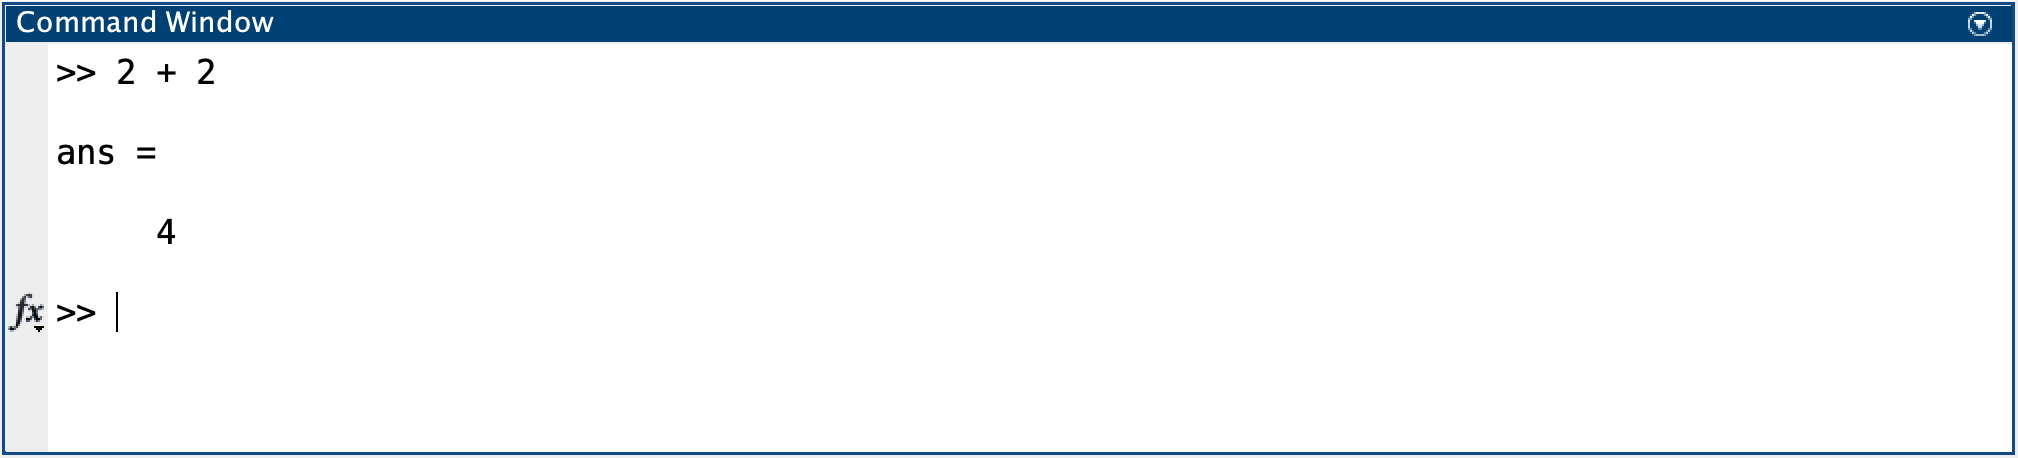
\includegraphics[width=0.95\textwidth]{Bilder/CommandWindow.png}}
                    \caption{Command Window in MATLAB}
                \end{figure}
                Im Command Window können Befehle direkt eingegeben werden. Da Ergebnisse von Berechnungen unverzüglich angezeigt werden, können hier einzelne Befehle idealerweise getestet werden.
            \subsubsection*{Editor}
                \begin{figure}[H]
                    \centering
                    \fbox{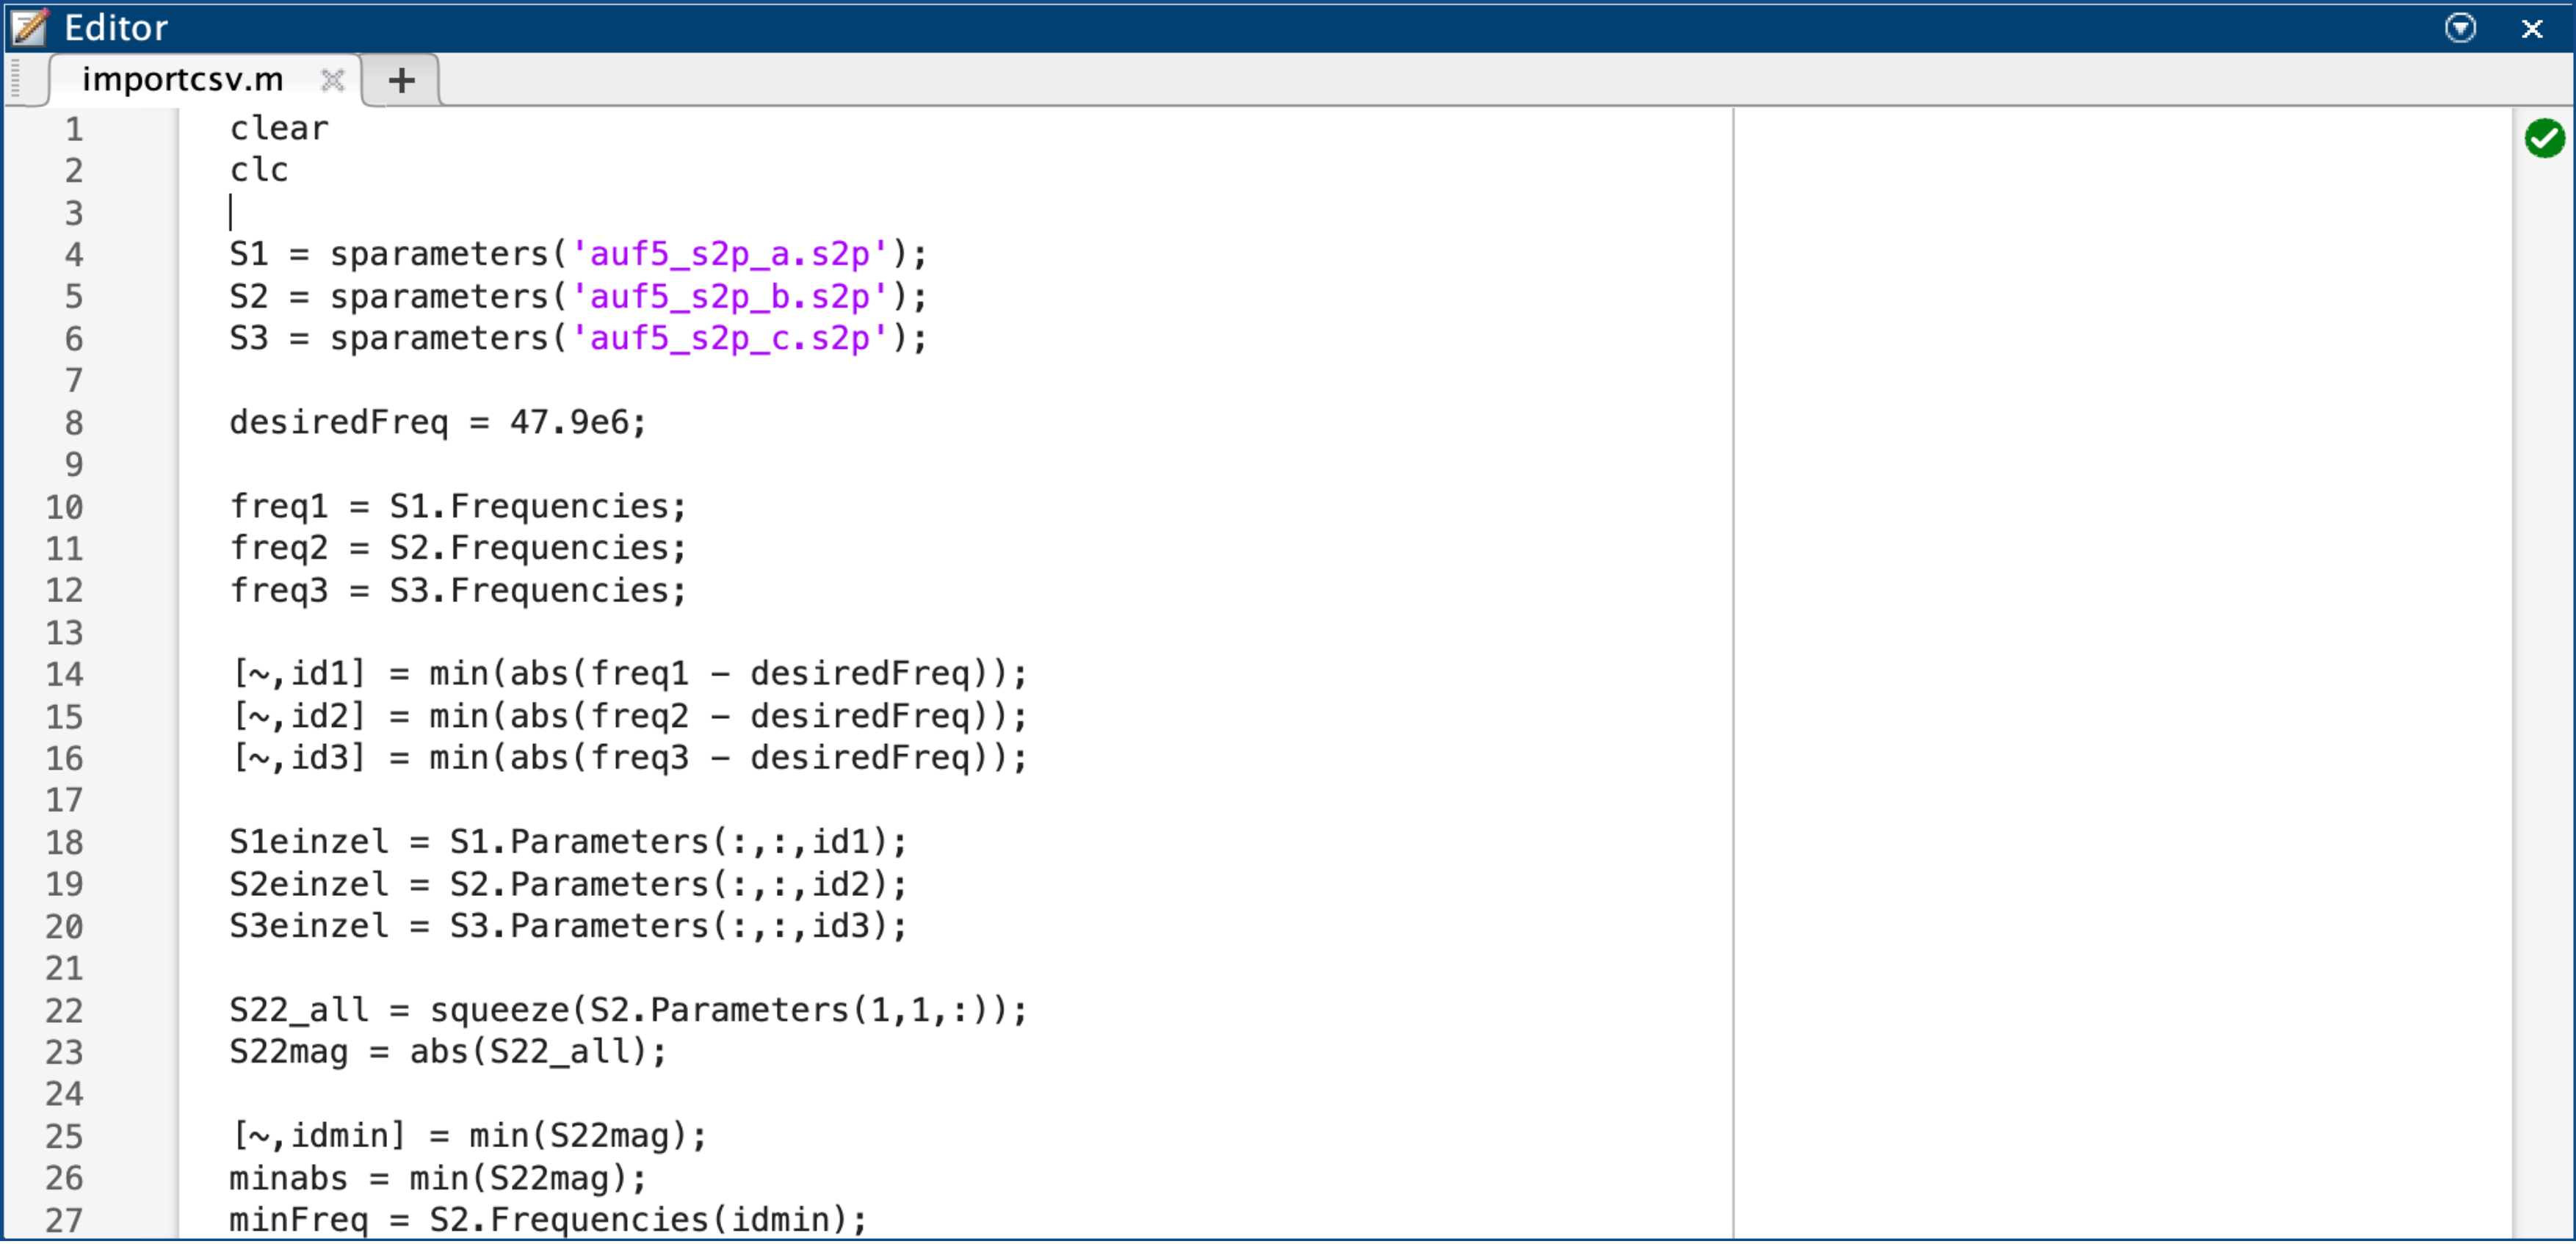
\includegraphics[width=0.95\textwidth]{Bilder/Editor.png}}
                    \caption{Editor in MATLAB}
                \end{figure}
                Im Editor können komplette Skripte und Funktionen geschrieben, gespeichert und ausgeführt werden. Er unterstützt das Debugging mittels Breakpoints und Schritt-für-Schritt Ausführung.
            \subsubsection*{Workspace}
                \begin{figure}[H]
                    \centering
                    \fbox{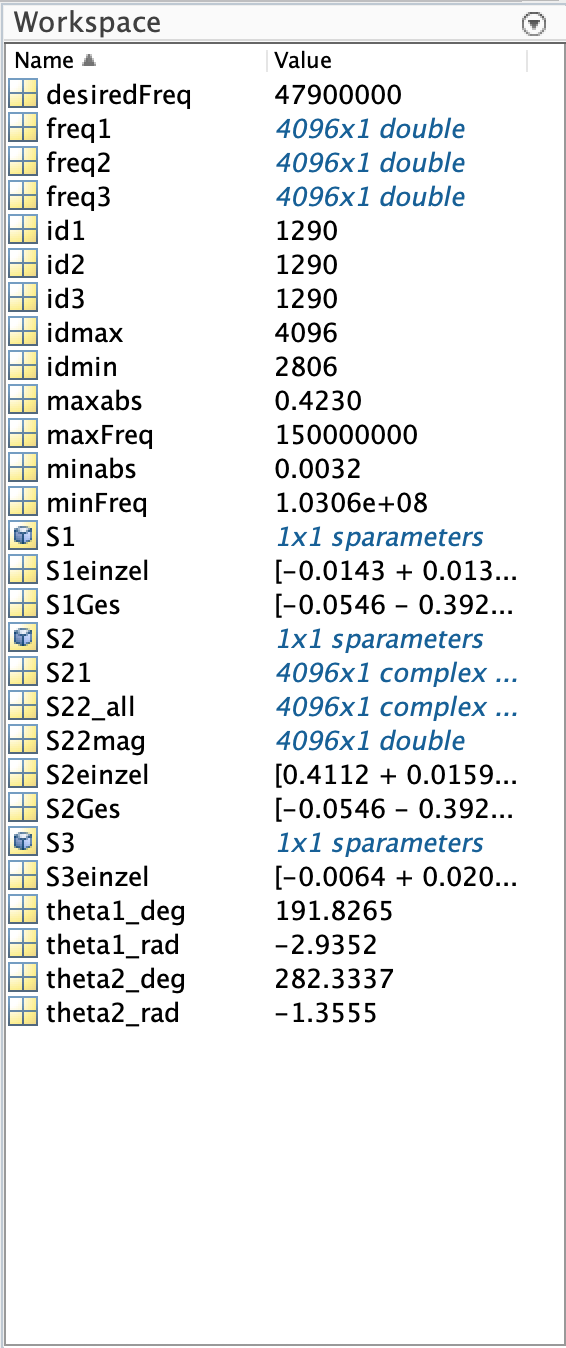
\includegraphics[width=0.2\textwidth]{Bilder/Workspace.png}}
                    \caption{Workspace in MATLAB}
                \end{figure}
                Im Workspace werden alle aktuellen Variablen inklusive ihres Inhalts angezeigt. Weiterhin ist es möglich diese Variablen hier manuell anzupassen oder zu löschen.
            \subsubsection*{Current Folder}
                \begin{figure}[H]
                    \centering
                    \fbox{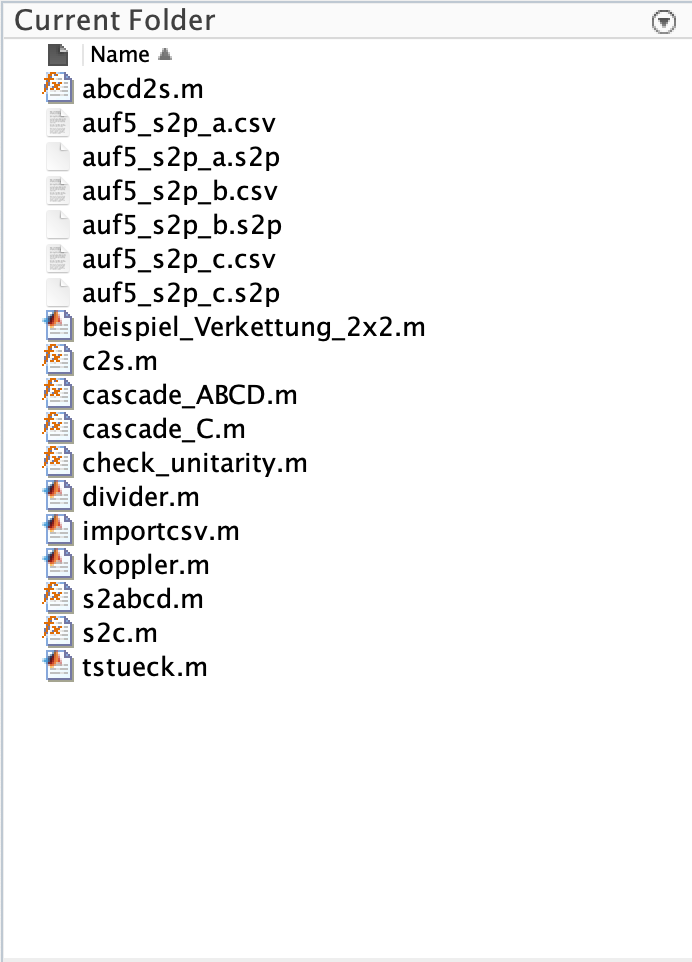
\includegraphics[width=0.3\textwidth]{Bilder/CurrentFolder.png}}
                    \caption{Current Folder in MATLAB}              
                \end{figure}
                Im Current Folder findet man alle Dateien des Projektordners. Diese können durch Doppelklick oder das Ziehen in den Editor geöffnet und bearbeitet werden.
            \newpage
            
    \section{Grundlegende Operationen}
        \subsection{Variablendeklaration}
                \begin{CodeErklaerungBox}{Einfache Wertzuweisung}
                \begin{lstlisting}
a = 3;
                \end{lstlisting}
                \tcblower
                Der Variable \texttt{a} wird der Wert \texttt{3} zugewiesen.
                \end{CodeErklaerungBox}
                \noindent Eine Zuweisung ohne ein Semikolon am Ende der Zeile bewirkt eine direkte Rückgabe des Variablenwertes.
                \begin{CodeErklaerungBox}{Fließkommazahl}
                \begin{lstlisting}
a = 4.5;
                \end{lstlisting}
                \tcblower
                Der Variable \texttt{a} wird der Wert \texttt{4.5} zugewiesen. Als Trennzeichen in MATLAB wird der Punkt an Stelle eines Kommas verwendet.
                \end{CodeErklaerungBox}
                \begin{CodeErklaerungBox}{Zeichenkette}
                \begin{lstlisting}
name = "Peter";
                \end{lstlisting}
                \tcblower
                Der Variable \texttt{name} wird der String \texttt{Peter} zugewiesen.
                \end{CodeErklaerungBox}
                \begin{CodeErklaerungBox}{Logischer Wert}
                \begin{lstlisting}
isValid = true;
                \end{lstlisting}
                \tcblower
                Der Variable \texttt{isValid} wird der boolsche Wert \texttt{true} zugewiesen.
                \end{CodeErklaerungBox}
                \begin{CodeErklaerungBox}{Automatische Typzuweisung}
                \begin{lstlisting}
a = pi;
                \end{lstlisting}
                \tcblower
                Der Variable \texttt{a} wird die, in MATLAB vordefinierte Variable $\pi$ zugewiesen.
                \end{CodeErklaerungBox}
                \noindent Neben pi gibt es weitere vordefinierte Variablen. Diesen kann zwar ebenfalls ein selbst definierter Wert zugewiesen werden, jedoch ist es nicht empfehlenswert.
                \begin{center}
                \renewcommand{\arraystretch}{1.4}
                \begin{tabularx}{\textwidth}{|l| X| l|}
                    \hline
                    \textbf{Variable} & \textbf{Bedeutung} & \textbf{Wert} \\
                    \hline
                    \texttt{inf} & Unendlich & $\frac{1}{0}$ ergibt \texttt{inf} \\
                    \hline
                    \texttt{i} & Imaginäre Einheit & $\sqrt{-1}$ \\
                    \hline
                    \texttt{j} & Alternative imaginäre Einheit & $\sqrt{-1}$ \\
                    \hline
                    \texttt{NaN} & "Not a Number" - ungültiger Wert & $\frac{0}{0}$ ergibt \texttt{NaN} \\
                    \hline
                    \texttt{ans} & Ergebnis der letzten berechneten Zeile & z.B. \texttt{ans = 42} \\
                    \hline
                    \texttt{true}/\texttt{false} & Boolsche Werte & \texttt{1} bzw. \texttt{0} \\
                    \hline
                \end{tabularx}
            \end{center}
        \subsection{Mathematische Grundoperationen}
            \begin{CodeErklaerungBox}{Addition}
                \begin{lstlisting}
c = a + b;
                \end{lstlisting}
                \tcblower
                In der Variable \texttt{c} wird die Summe aus \texttt{a} und \texttt{b} gespeichert.
                \end{CodeErklaerungBox}
                \begin{CodeErklaerungBox}{Subtraktion}
                \begin{lstlisting}
c = a - b;
                \end{lstlisting}
                \tcblower
                In der Variable \texttt{c} wird die Differenz aus \texttt{a} und \texttt{b} gespeichert.
                \end{CodeErklaerungBox}
                \begin{CodeErklaerungBox}{Multiplikation}
                \begin{lstlisting}
c = a * b;
                \end{lstlisting}
                \tcblower
                In der Variable \texttt{c} wird das Produkt aus \texttt{a} und \texttt{b} gespeichert.
                \end{CodeErklaerungBox}
                \begin{CodeErklaerungBox}{Division}
                \begin{lstlisting}
c = a / b;
                \end{lstlisting}
                \tcblower
                In der Variable \texttt{c} wird der Quotient aus \texttt{a} und \texttt{b} gespeichert.
                \end{CodeErklaerungBox}
                \begin{CodeErklaerungBox}{Abrunden}
                \begin{lstlisting}
c = floor(a / b);
                \end{lstlisting}
                \tcblower
                In der Variable \texttt{c} wird das abgerundete Ergebnis der Division von \texttt{a} und \texttt{b} gespeichert.
                \end{CodeErklaerungBox}
                \begin{CodeErklaerungBox}{Aufrunden}
                \begin{lstlisting}
c = ceil(a / b);
                \end{lstlisting}
                \tcblower
                In der Variable \texttt{c} wird das aufgerundete Ergebnis der Division von \texttt{a} und \texttt{b} gespeichert.
                \end{CodeErklaerungBox}
                \begin{CodeErklaerungBox}{Modulo}
                \begin{lstlisting}
c = mod(a,b);
                \end{lstlisting}
                \tcblower
                In der Variable \texttt{c} wird der Rest der Division von \texttt{a} und \texttt{b} gespeichert.
                \end{CodeErklaerungBox}
                \begin{CodeErklaerungBox}{Potenzieren}
                \begin{lstlisting}
c = a ^ 2;
                \end{lstlisting}
                \tcblower
                In der Variable \texttt{c} wird das Ergebnis der zweiten Potenz von \texttt{a} gespeichert.
                \end{CodeErklaerungBox}
                \begin{CodeErklaerungBox}{Wurzeln}
                \begin{lstlisting}
c = sqrt(a);
                \end{lstlisting}
                \tcblower
                In der Variable \texttt{c} wird die Wurzel von \texttt{a} gespeichert.
                \end{CodeErklaerungBox}
                \begin{CodeErklaerungBox}{Betrag}
                \begin{lstlisting}
c = abs(-a);
                \end{lstlisting}
                \tcblower
                In der Variable \texttt{c} wird der Betrag von \texttt{-a} gespeichert.
                \end{CodeErklaerungBox}
        \subsection{Komplexe Zahlen}
        \begin{CodeErklaerungBox}{Definition der komplexen Zahl}
                \begin{lstlisting}
z = 2 + 3*i;
                \end{lstlisting}
                \tcblower
                Erzeugt die komplexe Zahl \texttt{z = 2 + 3i}. 
                \end{CodeErklaerungBox}
                \noindent Wie unter 2.1 beschrieben, kann \texttt{j} analog zu \texttt{i} verwendet werden.
                \begin{CodeErklaerungBox}{Real- und Imaginärteil}
                \begin{lstlisting}
re = real(z);
im = imag(z);
                \end{lstlisting}
                \tcblower
                \texttt{real()} gibt den Realteil von \texttt{z} zurück und \texttt{imag()} den Imaginärteil.
                \end{CodeErklaerungBox}
                \begin{CodeErklaerungBox}{Betrag}
                \begin{lstlisting}
r = abs(z);
                \end{lstlisting}
                \tcblower
                Berechnet den Betrag von \texttt{z} , also $\sqrt{Im(z)^2 + Re(z)^2}$.
                \end{CodeErklaerungBox}
                \begin{CodeErklaerungBox}{Winkel}
                \begin{lstlisting}
phi = angle(z);
                \end{lstlisting}
                \tcblower
                Gibt den Winkel von \texttt{z} im Bogenmaß zurück.
                \end{CodeErklaerungBox}
                \begin{CodeErklaerungBox}{Konjugation}
                \begin{lstlisting}
z_conj = conj(z);
                \end{lstlisting}
                \tcblower
                Gibt das konjugiert Komplexe der Variable \texttt{z} also $z^* = Re(z) - i\cdot Im(z)$ zurück.
                \end{CodeErklaerungBox}
                \begin{CodeErklaerungBox}{Darstellung in Polarform}
                \begin{lstlisting}
r = abs(z);
phi = angle(z);
z_polar = r * exp(1i*phi);
                \end{lstlisting}
                \tcblower
                Gibt die komplexe Zahl \texttt{z} in Polarform zurück. \texttt{exp(1i * phi)} steht für $e^{i \cdot \phi}$
                \end{CodeErklaerungBox}
                \newpage
        \subsection{Beispielaufgaben}
                \subsubsection*{Aufgabe 1}
                Gegeben sei die Funktion $f(x) = x^2 +4x +5$. Berechnen Sie die komplexen Nullstellen der Funktion und lassen Sie sich jeweils Betrag und Phase ausgeben.
                \begin{Codelösung}{Lösung 1}
                    \begin{lstlisting}
p = 4;
q = 5;

x1 = -p/2 + sqrt((p/2)^2 - q);
x2 = -p/2 - sqrt((p/2)^2 - q);

r1 = abs(x1);
r2 = abs(x2);

phi1 = angle(x1);
phi2 = angle(x2);
                    \end{lstlisting}
                    
                \end{Codelösung}


                \subsubsection*{Aufgabe 2}
                Eine elektrische Schaltung besteht aus einem Widerstand mit $R=10\Omega$ einer Spule mit $L=0,05H$ und einem Kondensator mit $C=100\mu F$. Die Reihenschaltung der drei Elemente wird bei einer Frequenz von $f=50Hz$ betrieben. Berechnen Sie die Gesamtimpedanz $Z$ dieser Schaltung.
                \begin{Codelösung}{Lösung 2}
                    \begin{lstlisting}
R = 10;
L = 0.05;
C = 100e-6;
f = 50;
omega = 2 * pi * f;

Z_R = R;
Z_L = 1j * omega * L;
Z_C = 1 / (1j * omega * C);

Z_Gesamt = Z_R + Z_L + Z_C;
                    \end{lstlisting}   
                \end{Codelösung}
                
    \section{Vektoren und Matrizen}
        \subsection{Erstellen von Vektoren und Matrizen}
        \begin{CodeErklaerungBox}{Zeilenvektor}
                \begin{lstlisting}
v = [1 2 3 4];
                \end{lstlisting}
                \tcblower
                Erzeugt einen Zeilenvektor mit den angegebenen Werten. Statt der Trennung durch ein Leerzeichen können ebenfalls Kommata verwendet werden.
                \end{CodeErklaerungBox}
                \begin{CodeErklaerungBox}{Spaltenvektor}
                \begin{lstlisting}
v = [1;2;3;4];
                \end{lstlisting}
                \tcblower
                Erzeugt einen Spaltenvektor mit den angegebenen Werten.
            \end{CodeErklaerungBox}
            \begin{CodeErklaerungBox}{Doppelpunktoperator I}
                \begin{lstlisting}
v = x1:x2;
                \end{lstlisting}
                \tcblower
                Erzeugt einen Zeilenvektor von \texttt{x1} bis \texttt{x2} in ganzzahligen Schritten.
            \end{CodeErklaerungBox}
            \begin{CodeErklaerungBox}{Doppelpunktoperator II}
                \begin{lstlisting}
v = x1:step:x2;
                \end{lstlisting}
                \tcblower
                Erzeugt einen Zeilenvektor von \texttt{x1} bis \texttt{x2} in konstanten Schritten von \texttt{step}.
            \end{CodeErklaerungBox}
            \begin{CodeErklaerungBox}{linspace}
                \begin{lstlisting}
v = linspace(x1,x2,n);
                \end{lstlisting}
                \tcblower
                Erzeugt einen Zeilenvektor von \texttt{x1} bis \texttt{x2} mit \texttt{n} gleichmäßig verteilten Werten.
            \end{CodeErklaerungBox}
            \begin{CodeErklaerungBox}{Matrizen}
                \begin{lstlisting}
A = [1 2 3; 4 5 6; 7 8 9];
                \end{lstlisting}
                \tcblower
                Elemente einer Zeile der Matrix werden wie bei den Vektoren mit Leerzeichen oder Komma getrennt. Ein Zeilenumbruch erfolgt durch Eingabe eines Semikolon.
            \end{CodeErklaerungBox}
            \begin{CodeErklaerungBox}{0-Matrix}
                \begin{lstlisting}
A = zeroes(m,n);
                \end{lstlisting}
                \tcblower
                Erzeugt eine 0-Matrix der Größe \texttt{m}x\texttt{n}. \texttt{ones()} funktioniert analog zu \texttt{zeroes()} nur mit einsen.
            \end{CodeErklaerungBox}
            \begin{CodeErklaerungBox}{Einheitsmatrix}
                \begin{lstlisting}
A = eye(n);
                \end{lstlisting}
                \tcblower
                Erzeugt die Einheitsmatrix der Größe \texttt{n}x\texttt{n}.
            \end{CodeErklaerungBox}
        \subsection{Zugriff auf Elemente und Indizierung}
        \subsection{Matrixoperationen}
        \subsection{nützliche MATLAB Funktionen}
    \section{Programmiergrundlagen}
        \subsection{Skripte}
        \subsection{Funktionen}
        \subsection{Schleifen}
    \section{Arbeiten mit Dateien und Daten}
        \subsection{Speichern und Laden von Daten}
        \subsection{Importieren von Messdaten}
        \subsection{Analyse und Verarbeitung von Daten}
    \section{Visualisierung von Daten}
        \subsection{Einfache Diagramme}
        \subsection{Mehrere Kurven in einem Diagramm}
        \subsection{Mehrere Diagramme in einer Übersicht}
        \subsection{Grafische Anpassungen}
    \section{Anhang}
        \subsection{Dokumentation in MATLAB}
        \subsection{Übersicht wichtiger MATLAB Befehle}
\end{document}
